\documentclass[12pt]{article}

\usepackage{xeCJK}%字體設定
\setCJKmainfont{cwTeXKai}[AutoFakeBold=1.5]


\setmainfont{Times New Roman}  % 英文正文字體

\usepackage[top=2cm,bottom=2cm,left=2cm,right=2cm,a4paper]{geometry}%版面設定

\usepackage{indentfirst}%縮排

\usepackage{setspace}%行距設計
\onehalfspacing%半行距
\setlength{\parskip}{3pt}%段落之間

\usepackage{moresize}%字體大小

\usepackage{graphicx}

\usepackage{amssymb}%數學符號

\usepackage{amsmath} % 數學符號
\usepackage{booktabs}         % 漂亮的表格（\toprule, \midrule, \bottomrule）
\usepackage{siunitx}          % 國際單位制 (建議處理單位更漂亮)

\usepackage{multicol}%引入函數使下面那些可以變成雙欄

\usepackage{float}%圖片固定

% \renewcommand{\thesection}{\Roman{section}}


%%%%%%%%%%%%%%%%%%%%%%%%%%%%%%正文%%%%%%%%%%%%%%%%%%%%%%%%%%%%%%%%%%%
\begin{document}

\begin{titlepage}
\begin{center}

\vspace*{0.5cm}
\HUGE \textbf{普通物理實驗結報}\\
\vspace{2cm}
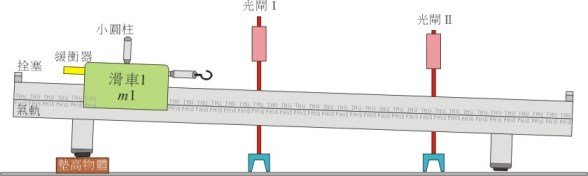
\includegraphics[width=15cm]{一維運動.jpg}\\[2cm]
\HUGE \textbf{一維運動}\\

\vfill
\huge 第三組\\[0.5cm]
\begin{table}[h]
\centering
\Large
\begin{tabular}{|c|c|}
\hline
組員:              & 貢獻度  \\
吳 & 33\% \\
卓 & 33\% \\
程 & 33\% \\ \hline
\end{tabular}
\end{table}

\end{center}

\end{titlepage}

%%%%%%%%%%%%%%%%%%%%%%%%%%%%%%%%%%%%%%%%%%%%%%%%%%%%%%%%%%%%%%%%

\large
\section{\textbf{實驗目的}}
透過牛頓第二定律求得重力加速度與驗證一維碰撞的動量守恆定律。

%%%%%%%%%%%%%%%%%%%%%%%%%%%%%%%%%%%%%%%%%%%%%%%%%%%%%%%%%%%%%%%%

\section{\textbf{實驗原理}}
物體質量 $( m ) $於斜角 $\theta$ 的斜面上，加速度沿斜面方向分量為gsin(theta)  
在一維碰撞中（無外力、無摩擦），系統動量守恆
%%%%%%%%%%%%%%%%%%%%%%%%%%%%%%%%%%%%%%%%%%%%%%%%%%%%%%%%%%%%%%
% \section{\textbf{理論分析}}

%%%%%%%%%%%%%%%%%%%%%%%%%%%%%%%%%%%%%%%%%%%%%%%%%%%%%%%%%%%%%%%%

\section{\textbf{實驗方法}}
利用光電閘與滑車系統，研究物體在無摩擦斜面上的加速度運動 
以LabQuest光電閘計時法測量瞬時速度與加速度
    

%%%%%%%%%%%%%%%%%%%%%%%%%%%%%%%%%%%%%%%%%%%%%%%%%%%%%%%%%%%%%%%%

\section{\textbf{數據分析}}
%%%%%%%%%%%%%%%%%%%%%%%%%實驗一%%%%%%%%%%%%
\subsection{實驗一:改變光電閘間距，計算重力加速度的大小。}

\begin{table}[H]
\centering
\resizebox{\textwidth}{!}{
\begin{tabular}{ccccccc}
\hline
\begin{tabular}[c]{@{}c@{}}光電閘間距\\ $X$ (cm)\end{tabular} &
\begin{tabular}[c]{@{}c@{}}滑車通過兩光電閘\\ 時間 $T$ (s)\end{tabular} &
\begin{tabular}[c]{@{}c@{}}通過光電閘1的\\ 時間 $\Delta t_1$ (s)\end{tabular} &
\begin{tabular}[c]{@{}c@{}}通過光電閘2的\\ 時間 $\Delta t_2$ (s)\end{tabular} &
\begin{tabular}[c]{@{}c@{}}通過光電閘1的\\ 速度 $V_1$ (m/s)\end{tabular} &
\begin{tabular}[c]{@{}c@{}}通過光電閘2的\\ 速度 $V_2$ (m/s)\end{tabular} &
\begin{tabular}[c]{@{}c@{}}斜面加速度\\ $a$ (m/s$^2$)\end{tabular} \\ \hline
20 & 0.2359 & 0.0146 & 0.0119 & 0.79 & 0.97 & 0.77 \\
30 & 0.3346 & 0.0144 & 0.0109 & 0.80 & 1.05 & 0.79 \\
40 & 0.4257 & 0.0144 & 0.0103 & 0.80 & 1.12 & 0.77 \\
50 & 0.5160 & 0.0144 & 0.0096 & 0.81 & 1.20 & 0.77 \\
60 & 0.6001 & 0.0145 & 0.0090 & 0.79 & 1.28 & 0.83 \\ \hline
重力加速度 $g$ (m/s$^2$)= & 9.65 &  &  &  &  &  \\
$\sin\theta$= & 0.085 & 斜面長度= & 130 cm & 斜面高度= & 11 cm &  \\ \hline
\end{tabular}
}
\caption{光電閘測量滑車加速度實驗數據}
\label{tab:glider}
\end{table}


\begin{itemize}
    \item 我們推測在該實驗中，可能的誤差來源有：
        \begin{enumerate}
          \item 光電閘間距越大，包含到斜面不平整的地方。
          \item 滑車是以車輪滾動前進的而不是像理論中所假設的滑動向下。
          \item 滑車上的遮光片傾斜。
        \end{enumerate}
    \item 首先，觀察光電閘間距60cm的實驗數據，發現相比其餘四組實驗所求得的加速度相差較大，也因為我們每組實驗都有重複三次，所以可以排除60cm所測得的數據為乖離值，再來20～50cm實驗組加速度並未出現太大的跳動，也就可以推測，我們使用的斜面，可能在從光電閘1向下50至60cm並不平整，存在顛簸、凸起的情況。
    \item 若考慮車輪滾動，是否對於計算重力加速度有誤差?\\
    已知:
    \[
    g = \frac{M_{\text{tot}}+2M_w}{M_{\text{tot}}\sin\theta}  a
    \]
    首先，因為我們沒辦法把車輪拔下來秤重，所以不妨假設一個車輪重1公克，而滑車重量經過測量為391.16公克，將這些代入誤差公式：
    \[
    Error=\frac{2\times0.001}{0.39116+0.006}=0.5\%
    \]
    由此可知該因素並不會造成很大的誤差，所以在接下來的討論中將不再強調。\\
    （$\ast$ 公式推導部分請見附錄：考慮車輪滾動但不滑動的修正推導）

    \item 因為不能保證遮光片與滑軌是處於平行，所以我們算出了遮光片傾斜後可能造成的誤差，那將一些角度代入後得到下表：
    \begin{table}[H]
    \centering
\begin{tabular}{cc}
\hline
\begin{tabular}[c]{@{}l@{}}$\theta$(deg)\end{tabular} & $1-\cos^2 \theta$ \\ \hline
1                                                                     & 0.03\%            \\
3                                                                     & 0.20\%            \\
5                                                                     & 0.76\%            \\
7                                                                     & 1.49\%            \\
9                                                                     & 2.45\%            \\
10                                                                    & 3.02\%             \\ \hline
\end{tabular}
\end{table}
在實驗中應該不至於有大於5度的落差，所以遮光片傾斜不會對實驗數據有過多的影響。\\
 （$\ast$ 公式推導部分請見附錄：滑車上遮光板影響）

 \item 綜上所述，該實驗中比較可能的誤差來源主要應該為部分斜面不平整導致，次因則是遮光片傾斜的問題。
\end{itemize}




%%%%%%%%%%%%%%%%%%%%%%%%%%%%%%實驗二%%%%%%%
\subsection{實驗二:改變斜面傾斜的角度，計算重力加速度大小}

\begin{table}[H]
\centering
\resizebox{\textwidth}{!}{
\begin{tabular}{ccccc}
\hline
\begin{tabular}[c]{@{}c@{}}斜面傾斜角度\\ (deg)\end{tabular} &
\begin{tabular}[c]{@{}c@{}}滑車通過光電閘1的速度\\ $V_1$ (m/s)\end{tabular} &
\begin{tabular}[c]{@{}c@{}}滑車通過光電閘2的速度\\ $V_2$ (m/s)\end{tabular} &
\begin{tabular}[c]{@{}c@{}}滑車加速度\\ $a$ (m/s$^2$)\end{tabular} &
\begin{tabular}[c]{@{}c@{}}重力加速度\\ $g$ (m/s$^2$)\end{tabular} \\ \hline
5.56 & 0.90 & 1.43 & 1.02 & 9.81 \\
3.44 & 0.67 & 1.06 & 0.56 & 9.33 \\ \hline
平均重力加速度 $\bar{g}$ = & 9.57 (m/s$^2$) &  &  &  \\ \hline
\end{tabular}
}
\caption{不同斜面角度下滑車速度與重力加速度測量值}
\label{tab:gravity}
\end{table}

\begin{itemize}
    \item 在此實驗中，因為實驗器材與實驗一雷同，所以部分誤差來源相同，例:斜面平整度、遮光板傾斜。但在此實驗中，操縱變因是改變斜面傾斜角度，所以會有更大的人為誤差，例如:人眼對齊直尺刻度、需要延伸斜面來計算$\sin\theta$等等。
\end{itemize}





%%%%%%%%%%%%%%%%%%%%%%%%%%實驗三%%%%%%%%%%%
\subsection{實驗三:執行彈性/非彈性/完全非彈性碰撞，觀察滑車動量}

\begin{table}[H]
\centering
\resizebox{\textwidth}{!}{
\begin{tabular}{cccccccc}
\hline
碰撞類型 &
\begin{tabular}[c]{@{}c@{}}滑車A通過光電閘1\\ 時間 $\Delta t_A$ (s)\end{tabular} &
\begin{tabular}[c]{@{}c@{}}滑車B通過光電閘2\\ 時間 $\Delta t_B$ (s)\end{tabular} &
\begin{tabular}[c]{@{}c@{}}滑車A通過光電閘2\\ 時間 $\Delta t_A'$ (s)\end{tabular} &
\begin{tabular}[c]{@{}c@{}}滑車A初速度\\ $V_A$ (m/s)\end{tabular} &
\begin{tabular}[c]{@{}c@{}}滑車A末速度\\ $V_A'$ (m/s)\end{tabular} &
\begin{tabular}[c]{@{}c@{}}滑車B末速度\\ $V_B'$ (m/s)\end{tabular} &
\begin{tabular}[c]{@{}c@{}}碰撞前後動量比值\\ $\frac{P'}{P_0}$\end{tabular} \\ \hline
彈性碰撞 & 0.01752 & 0.01758 & / & 0.66 & / & 0.65 & 0.996 \\
完全非彈性碰撞 & 0.01960 & 0.03804 & 0.03804 & 0.59 & 0.30 & 0.30 & 1.030 \\ \hline
$M_A=$ & 391.31 g &  &  &  &  &  &  \\
$M_B=$ & 391.16 g &  &  &  &  &  &  \\ \hline
\end{tabular}
}
\caption{不同碰撞類型下滑車速度與動量比值}
\label{tab:collision}
\end{table}






\subsubsection{彈性碰撞}
\begin{itemize}
    \item 在此實驗中，系統碰撞前與碰撞後動量並明顯差異的，此結果也是符合預期，因為A、B兩滑車並無受到外力作用，所以系統動量守恆。
    \item 實驗中可能誤差為橡皮筋若沒有繃緊，可能使碰撞變為非彈性碰撞。
\end{itemize}

\subsubsection{完全非彈性碰撞}
\begin{itemize}
    \item 在此實驗中，系統碰撞前與碰撞後動量並明顯差異的，此結果也是符合預期，因為A、B兩滑車並無受到外力作用，所以系統動量守恆。
\end{itemize}


%%%%%%%%%%%%%%%%%%%%%%%%%%實驗四%%%%%%%%%%%

\subsection{\textbf{實驗四}:計算斜面摩擦係數}
\begin{table}[H]
\centering
\begin{tabular}{cccc}
\hline
\begin{tabular}[c]{@{}c@{}}斜面角度\\ $\theta(deg)$\end{tabular} & $sin \theta$ & \begin{tabular}[c]{@{}c@{}}滑車加速度\\ $a( m/s^2)$\end{tabular} & \begin{tabular}[c]{@{}c@{}}動摩擦係數\\ $\mu_k$\end{tabular} \\ \hline
3.44                                                         & 0.06         & 0.560                                                       & 0.0020                                                  \\
5.74                                                         & 0.1          & 0.722                                                       & 0.0253                                                  \\ \hline
\end{tabular}
\caption{斜面動摩擦力}
\label{tab:摩擦力}
\end{table}
\begin{itemize}
    \item 我們該組實驗會出現將近十倍的誤差，主要原因是我們斜面的角度過小，導致在實驗二提到的$\sin\theta$量測不精確的誤差更為明顯。
\end{itemize}


\subsubsection{小角度下誤差放大的分析}
\noindent
本實驗使用公式：
\[
\mu_k = \frac{g\sin\theta - a}{g\cos\theta},
\]
其中 $\theta$ 為斜面角度、$a$ 為滑車加速度、$g$ 為重力加速度。  
以實驗數據代入：
\[
\begin{aligned}
\theta &= 3.44^\circ, \quad a = 0.560\ \mathrm{m/s^2}, \\
\theta &= 5.74^\circ, \quad a = 0.722\ \mathrm{m/s^2}, \\
g &= 9.65\ \mathrm{m/s^2},
\end{aligned}
\]
可得：
\[
\mu_k(3.44^\circ) \approx 0.0020, \qquad
\mu_k(5.74^\circ) \approx 0.0253.
\]
可以發現第一組結果異常地接近零。其原因在於小角度時
$\sin\theta$ 的數值極小，使得分子
$g\sin\theta - a$ 的差值非常敏感，
任何微小的量測誤差都會被放大。

\noindent
\textbf{例如：}
以 $\theta = 3.44^\circ, a = 0.560$ 為例：

\begin{itemize}
    \item 角度改變 $\pm0.1^\circ$：
    \[
    \mu_k(3.54^\circ) \approx 0.00467, \qquad
    \mu_k(3.34^\circ) \approx 0.00118,
    \]
    相差約四倍。
    \item 加速度改變 $\pm0.02\ \mathrm{m/s^2}$：
    \[
    \mu_k(a=0.580) \approx 0.00088, \qquad
    \mu_k(a=0.540) \approx 0.00497,
    \]
    僅 $0.02\ \mathrm{m/s^2}$ 的誤差便使結果變化數倍。
\end{itemize}

因此，小角度下的摩擦係數計算極為不穩定，微小的角度或加速度誤差皆可能導致 $\mu_k$ 偏離實際值數倍。
這情況並非公式出錯，而是數值在小角度下變化劇烈所導致。

\vspace{1em}
\noindent
所以，在小角度 ($\theta < 5^\circ$) 的情況下，
$\sin\theta$ 與 $a$ 的量測誤差會被放大，
導致 $\mu_k$ 數值波動劇烈甚至出現負值。
如果要降低此影響，可採取以下策略來調整實驗步驟：

\begin{enumerate}
    \item 使用較大角度（$8^\circ$–$15^\circ$）進行量測，以降低誤差敏感度。
    \item 提高角度量測精度，例如以傾角計或高度比 $h/L$ 方式求 $\sin\theta$。
    \item 以「恆速滑行法」量得 $\mu_k = \tan\theta$，避免使用加速度測值。
\end{enumerate}

綜上所述，第一組實驗中摩擦係數極小的結果，
主要源自小角度下的量測誤差放大效應，
而非實際摩擦力趨近於零。








\newpage
%%%%%%%%%%%%%%%%%%%%%%%%%%%%%%%%%%%%%%%%%%%%%%%%%%%%%%%%%%%%%%%%

\section{\textbf{結果與討論}}

As a whole, the experiment has been a success. From the slope test to the collision test, the results were very satisfying, almost matching the expected theoretical values. \\

Experiment 1 involved the slope test, designed to determine whether acceleration is truly affected by gravity, using the formula $a=g\times\sin\theta$. Our results aligned well with the theory, with only tiny, negligible discrepancies.\\

Experiment 2 performed just as well. The total momentum in our experiment followed the law of momentum conservation for both elastic and inelastic collisions. In the elastic collision, one cart bounced away while the other came to a stop, as expected since their masses were equal. In the inelastic collision, the after-collision momentum was roughly half of the before-collision momentum, consistent with theoretical predictions.\\

Although our friction calculations may have been slightly skewed, this was likely due to skipping wheels and minor inaccuracies in measurement. Small changes in these factors can produce significant differences in the measured acceleration, making the effective μ value quite sensitive to slight variations.
%%%%%%%%%%%%%%%%%%%%%%%%%%%%%%%%%%%%%%%%%%%%%%%%%%%%%%%%%%%%
\newpage
\section*{附錄:考慮車輪滾動但不滑動的修正推導}
\noindent
假設滑車質量為 $M_{\text{car}}$，四個輪子的質量為 $M_w$、半徑為 $R_w$，輪子的轉動慣量為:
\[
I = \frac{1}{2} M_w R_w^2
\]
則滑車總質量為
\[
M_{\text{tot}} = M_{\text{car}} + 4M_w
\]

\begin{enumerate}

    \item \textbf{平移運動方程：}  
    滑車受重力沿斜面分力與摩擦力作用，有
    \[
        M_{\text{tot}} a = M_{\text{tot}} g \sin\theta - 4 f_i
    \]
    其中 $f_i$ 為單一輪子受到的摩擦力。

    \item \textbf{輪子轉動方程：} 
    對每個輪子取力矩：
    \[
    \tau = I \alpha = f_i R_w
    \]
    由於無滑動條件 $\alpha = \frac{a}{R_w}$，代入得
    \[
    f_i = \frac{I a}{R_w^2} = \frac{1}{2} M_w a
    \]

    \item \textbf{聯立方程：}
    將 $f_i$ 代入平移運動式：
    \[
    M_{\text{tot}} a = M_{\text{tot}} g \sin\theta - 4 \left( \frac{1}{2} M_w a \right)
    \]
    化簡得
    \[
    (M_{\text{tot}} + 2M_w)a = M_{\text{tot}} g \sin\theta
    \]
    \[
    \Rightarrow \boxed{g = \frac{M_{\text{tot}}+2M_w}{M_{\text{tot}}\sin\theta}  a}
    \] 

    \item \textbf{與原先方程式之誤差公式}
    \[
    Error= \frac{g_0-g}{g}=\frac{2M_w}{M_{\text{tot}}+2M_w}
    \]
    

    \item \textbf{靜摩擦條件:} 
    若輪子不滑動，則需滿足
    \[
    f_i \le \mu_s N_i
    \]
    其中 $N=M_{\text{tot}} g \cos\theta$。代入 $f_i = \frac{1}{2} M_w a$ 得
    \[
    \mu_s \ge \frac{M_w a}{2M_{\text{tot}} g \cos\theta}
    \]

\end{enumerate}


\section*{滑車上遮光板影響}
\noindent
考慮滑車上遮光板與前進方向存在一個傾斜角度$\theta$，這會導致我們量測的遮光板長度與實際通過光電閘測得的速度出現誤差。假設遮光板長度為$\Delta x$、通過光電閘1的時間為$\Delta t_1$、通過光電閘2的時間為$\Delta t_2$、兩光電閘間距為$L$。

\begin{enumerate}
    \item 遮光板不傾斜情況下的加速度
    \[
    a=\frac{(\frac{\Delta x}{\Delta t_2})^2-(\frac{\Delta x}{\Delta t_1})^2}{2L}
    \]
    \item 加入傾斜角度的情況下，加速度會變為：
    \[
    a^\prime=\frac{(\frac{\Delta x\cos \theta}{\Delta t_2})^2-(\frac{\Delta x \cos \theta}{\Delta t_1})^2}{2L} 
    \]
    \item 計算誤差
    \[
    Error=\frac{a-a^\prime}{a}=1-\cos^2 \theta
    \]
    接著可以代入一些角度，觀察誤差的大小。
    
\end{enumerate}
%%%%%%%%%%%%%%%%%%%%%%%%%%%%%%%%%%%%%%%%%%%%%%%%%%%%%%%%%%%%%%%%%%%



\end{document}